\documentclass[border=8pt]{standalone}
\usepackage{tikz}
\usetikzlibrary{arrows.meta,positioning,calc}
\begin{document}
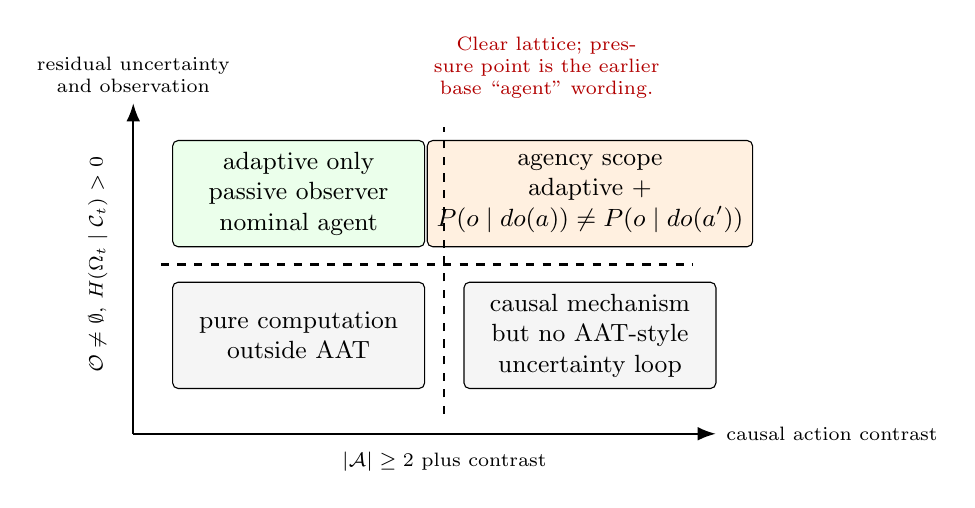
\begin{tikzpicture}[
  cell/.style={draw, rounded corners=2pt, minimum width=3.2cm, minimum height=1.35cm, align=center, font=\small},
  axis/.style={-Latex, thick},
  note/.style={align=center, font=\scriptsize}
]

\draw[axis] (0,0) -- (7.4,0) node[right, note] {causal action contrast};
\draw[axis] (0,0) -- (0,4.2) node[above, note] {residual uncertainty\\and observation};

\node[cell, fill=gray!8] at (2.1,1.25) {pure computation\\outside AAT};
\node[cell, fill=green!8] at (2.1,3.05) {adaptive only\\passive observer\\nominal agent};
\node[cell, fill=orange!12] at (5.8,3.05) {agency scope\\adaptive +\\$P(o\mid do(a))\ne P(o\mid do(a'))$};
\node[cell, fill=gray!8] at (5.8,1.25) {causal mechanism\\but no AAT-style\\uncertainty loop};

\draw[dashed, thick] (3.95,0.25) -- (3.95,3.9);
\draw[dashed, thick] (0.35,2.15) -- (7.1,2.15);

\node[note] at (3.95,-0.35) {$|\mathcal A|\ge2$ plus contrast};
\node[note, rotate=90] at (-0.45,2.15) {$\mathcal O\ne\emptyset$, $H(\Omega_t\mid\mathcal C_t)>0$};

\node[note, red!70!black, text width=4.0cm] at (5.25,4.65) {Clear lattice; pressure point is the earlier base ``agent'' wording.};

\end{tikzpicture}
\end{document}
